\documentclass{standalone}
\usepackage{tikz}
\usepackage{ctex,siunitx}
\usepackage{tkz-euclide}
\usepackage{amsmath}
\usetikzlibrary{patterns, calc}
\usetikzlibrary {decorations.pathmorphing, decorations.pathreplacing, decorations.shapes,}
\begin{document}
\small
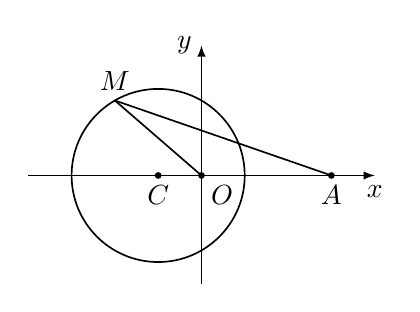
\begin{tikzpicture}[>=latex,scale=0.55]
  \draw[thin,->](-4,0)--(4,0)node[below]{$x$};
  \draw[thin,->](0,-2.5)--(0,3)node[left]{$y$};
  \tkzDefPoints{0/0/O,3/0/A,-1/0/C}
  \tkzDefShiftPoint[C](120:2){M}
  \tkzDrawCircle[semithick,black](C,M)
  \tkzDrawSegments[semithick](M,O M,A)
  \tkzDrawPoints[fill=black](A,O,C)
  \tkzLabelPoints[above](M)
  \tkzLabelPoints[below](A,C)
  \tkzLabelPoints[below right](O)
\end{tikzpicture}
\end{document}